\section{Hardware Timer Example}

\subsection{Introduction}\label{demo-intro}
This section describes the demonstrator system which uses a timer in programmable logic for generating interrupts on the Xilinx Zynq platform.


\subsection{Prerequisites}
The demonstrator system has been implemented on the Digilent Zybo Z7-20 board with Xilinx Vivado 2018-3.
If you want to use the demonstrator system directly, the aforementioned board is required with a Vivado installation containing the board support package.
Any Vivado installation \emph{should} work.
If you use a Zybo Z7 board, a Vivado version 2018.x and later is more convenient since you will not have to backport devicetrees and menuconfig when building the Linux image.
See Appendix~\ref{Vivado-bitstream} if you want to use a different board or are interested in how to manually build the system on the FPGA for generating the bitstream.

Debian 9 with Linux kernel 4.19 is used as the Linux image on the Zybo board, which boots from a micro SD card.
The image has been built using this \cite{DebianImage} guide.
See Appendix~\ref{Linux-Image} for details regarding the Linux image.

The prerequisites can be summarized as follows:
\begin{itemize}
\item Vivado installation (version 2017.x and later /emph{should} work)
\item A evaluation board with a Zynq 7000 chip (e.g. ZedBoard, MicroZed, Zybo, Zybo Z7)
\item Board support package for the board to be used in Vivado
\end{itemize}

\subsection{Hardware Implementation}


\subsection{Linux Kernel}\label{kernel}
%"Documentation/devicetree/bindings/interrupt-controller/arm,gic.yaml"

%kernel version: 4.19
% commit on linux-xlnx: 0ee2ead168af335315b6cd8c55cbf6e45998f585
% commit on u-boot-xlnx: 195c620e348891ca2d90c759781413f2adb3f748

\subsection{Linux User Space}

\subsubsection{Generating Interrupts}

The user space application for using the kernel module is pretty straight forward.
It can be compiled using the provided Makefile on either the host platform (using the Xilinx cross-compile tool-chain) or directly on the target.
The Xilinx environment has to be sourced first for cross compiling.
Otherwise, just copy the Makefile and timer.c file on the target (e.g. Zybo Z7 board) or use a different method such as \emph{sshfs} to mount a directory of your host on the target.

The kernel module can be compiled in the same way as the user program.

As a first step, load the kernel module as shown in figure~\ref{fig:enable-logic}.
The output of \emph{dmesg} should show that the kernel module has been loaded successfully.

\begin{figure}[ht]
    \centering
    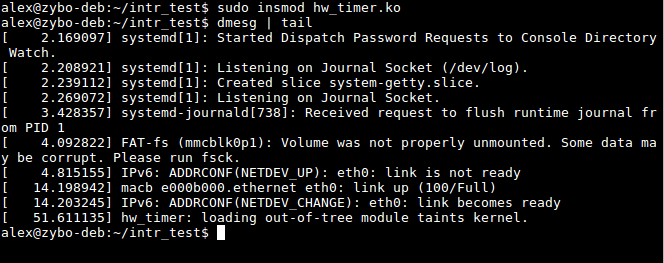
\includegraphics[width=1.0\textwidth,height=1.0\textheight,keepaspectratio]{figures/loaded_driver.png}
    \caption{Loading the kernel module}
    \label{fig:enable-logic}
\end{figure}

Figure~\ref{interrupt-list} shows the available interrupts for all CPUs.
The interrupt for our timer has been registered with number 45 in the list.
The actual interrupt number is displayed as 61 and is triggered on a (positive) edge.
The zeroes at the CPU columns indicate that no interrupt has been generated yet.

\begin{figure}[ht]
    \centering
    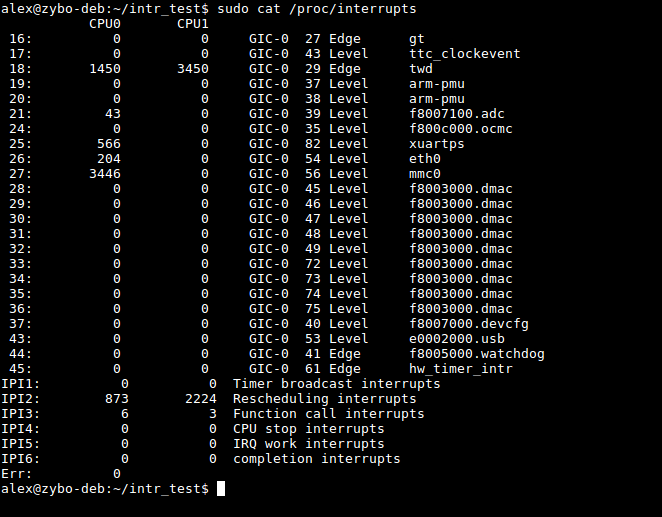
\includegraphics[width=1.0\textwidth,height=1.0\textheight,keepaspectratio]{figures/interrupt_entry.png}
    \caption{List of interrupts before generating timer interrupts}
    \label{fig:interrupt-list}
\end{figure}

Executing the test program compiled from timer.c gives the output shown in figure~\ref{fig:user-program}.

\begin{figure}[ht]
    \centering
    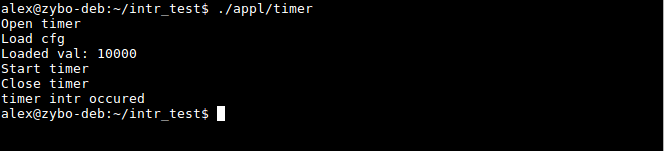
\includegraphics[width=1.0\textwidth,height=1.0\textheight,keepaspectratio]{figures/execute_user.png}
    \caption{Output of user program interfacing the kerne module}
    \label{fig:user-program}
\end{figure}

Looking at the list of interrupts again should now display a one for the column of CPU0 as shown in figure~\ref{fig:generated-interrupt}.

\begin{figure}[ht]
    \centering
    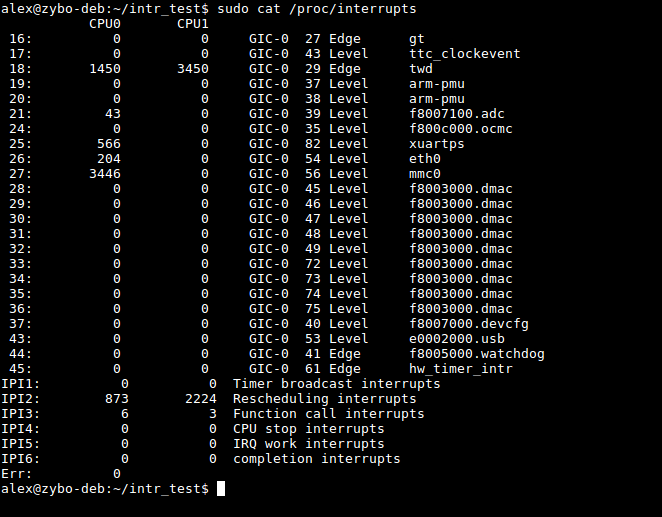
\includegraphics[width=1.0\textwidth,height=1.0\textheight,keepaspectratio]{figures/interrupt_entry.png}
    \caption{List of interrupts before generating timer interrupts}
    \label{fig:generated-interrupt}
\end{figure}

\subsubsection{Access Permissions}
It may be necessary to execute the user program with privileged access righs (using sudo).
If the device added by the kernel module should also be accessible by other users, a udev rule can be added to change permissions automatically when the device is added to the file system.
Figure~\ref{fig:udev-rule} shows the content of the rule and its path on the file system.
Just create a new file containing the shown content.

\begin{figure}[ht]
    \centering
    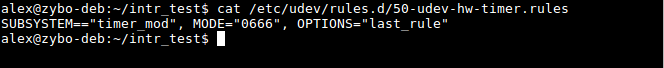
\includegraphics[width=1.0\textwidth,height=1.0\textheight,keepaspectratio]{figures/udev_rule.png}
    \caption{Changing device permissions}
    \label{fig:udev-rule}
\end{figure}

The udev rule should change permissions to the \emph{/dev/timer\_dev} as shown in figure~\ref{fig:file-permission}.

\begin{figure}[ht]
    \centering
    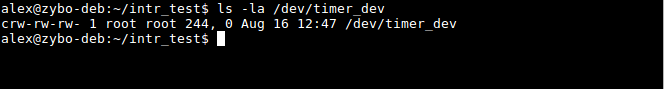
\includegraphics[width=1.0\textwidth,height=1.0\textheight,keepaspectratio]{figures/device_permission.png}
    \caption{Device permission after adding udev rule}
    \label{fig:file-permission}
\end{figure}

Figure~\ref{fig:device-info} shows how obtain the \emph{SUBSYSTEM} of the kernel module in case you want to add a similar udev rules for other devices.
\begin{figure}[ht]
    \centering
    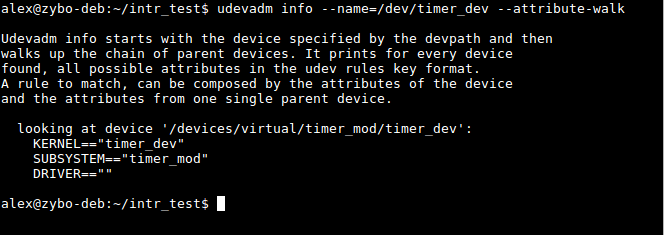
\includegraphics[width=1.0\textwidth,height=1.0\textheight,keepaspectratio]{figures/device_info.png}
    \caption{Getting detailed information for target device}
    \label{fig:device-info}
\end{figure}
